% Created 2021-03-18 Thu 21:23
% Intended LaTeX compiler: pdflatex
\documentclass[11pt]{article}
\usepackage[utf8]{inputenc}
\usepackage[T1]{fontenc}
\usepackage{graphicx}
\usepackage{grffile}
\usepackage{longtable}
\usepackage{wrapfig}
\usepackage{rotating}
\usepackage[normalem]{ulem}
\usepackage{amsmath}
\usepackage{textcomp}
\usepackage{amssymb}
\usepackage{capt-of}
\usepackage{hyperref}
\author{Dominik Pegler}
\date{\today}
\title{Aufgabe A1\\\medskip
\large Beispiele für gute und schlechte Bedienoberflächen}
\hypersetup{
 pdfauthor={Dominik Pegler},
 pdftitle={Aufgabe A1},
 pdfkeywords={},
 pdfsubject={},
 pdfcreator={Emacs 27.1 (Org mode 9.4.4)}, 
 pdflang={English}}
\begin{document}

\maketitle
\tableofcontents
\section{Aufgabe}
\label{sec:orge72ece6}
\begin{enumerate}
\item Recherchieren Sie nach drei, aus Ihrer Sicht, guten und drei
schlechten Bedienoberflächen:
\begin{enumerate}
\item jeweils eine mobile App
\item eine Webseite
\item und ein anderweitiges Beispiel (wie z.B. die eines Automaten,
Gerätes, einer Anlage, etc.), also abseits typischer Computer
oder mobiler Geräte.
\end{enumerate}
\item Begründen Sie aus ihrer persönlichen Sicht, warum Sie diese
Bedienoberflächen als gut bzw. als schlecht einstufen und zeigen
Sie dazu Fotos oder Screenshots, die Ihre Begründungen
untermauern.
\item Wählen sie ein von Ihnen als schlecht bewertete Bedienoberfläche
oder Website aus:
\begin{enumerate}
\item Analysieren sie diese Seite/Oberfläche basierend auf den in der
VU durchgenommenen Nielsen Heuristiken.
\item Schlagen Sie zwei wesentliche Verbesserungen vor.
\end{enumerate}
\end{enumerate}

\section{Beantwortung}
\label{sec:org177b5f8}

\subsection{3 gute, 3 schlechte Bedienoberflächen}
\label{sec:orgf9887ee}
\subsubsection{Gute Bedienüberflächen}
\label{sec:orgc5556c5}

\begin{enumerate}
\item Mobile: oebb.at
\item Web: MS Teams
\item Andere: Boxautomaten im Wiener Prater
\end{enumerate}

\subsubsection{Schlechte Bedienoberflächen}
\label{sec:org4999a2a}


\begin{enumerate}
\item Mobil: iOS Wecker
\item Web: gmx.at
\item Andere: Fahrkartenautomaten in verschiedenen europäischen Städten
\end{enumerate}

\subsection{Begründung}
\label{sec:org7dab56a}

Ich möchte hier den Fokus auf verbesserungswürdige Interfaces legen.

Obwohl gmx.at sicherlich nicht eine der schlechteste Webseiten ist,
vor allem weil das Hauptziel der Seite wahrscheinlich nicht darin
besteht, für die Benutzer des Email-Dienstes dazusein, finde ich
die Seite als Webmail-Dienst nicht besonders gut. Das Wichtigste
aus dieser Perspektive ist der Zugang zu den Emails und dieser
Funktion, obwohl zentral auf der Seite platziert, wird durch einen
Cluttermix an Distraktoren wie Werbung und Nachrichtenmeldungen die
Aufmerksamkeit des Benutzers vorenthalten.

Die Wecker-Funktion innerhalb der iOS-Uhr-Applikation finde ich
nicht sehr intuitiv. Die App scheint optimiert darauf zu sein,
voreingestellte Wecker-Zeiten an- und auszuschalten. Möchte man
jedoch eine dieser Wecker-Zeiten ändern, muss man am oberen linken
Bildschirmrand eine Schaltfläche berühren, die dann die App in eine
Art "Editiermodus" versetzt. In diesem kann man dann alle
Weckerzeiten ändern. Meist geht es aber nur darum eine einzelne
Zeit zu ändern und die erste, intuitive Reaktion ist immer, direkt
die Zeit am Touchscreen zu berühren. Hinter dieser Geste liegt
jedoch keine Funktion.

Viele moderne Fahrkartenautomaten berücksichtigen schon wichtige
Design-Prinzipien. Was jedoch noch zu wenig einfließt, ist der
Umstand, dass die Mobilität zwischen den Ländern in den letzten
Jahrzehnten stark zugenommen hat. Jeder dieser Fahrkartenautomaten
spricht seine eigene "Sprache", in sich logisch, jedoch nicht
kompatibel mit Personen, die mit den Fahrkartenautomaten und deren
Eigenheiten in anderen Städten und Ländern vertraut sind. Eine
einheitliche Linie bei der Gestaltung im Sinne einer Kooperation
unter den Staaten (z.B. EU) wäre meiner Meinung nach sinnvoll. Das
betrifft auch die mobilen Apps und Webseiten.

\subsection{Analyse einer schlechten Bedienoberfläche}
\label{sec:orgf0a6343}

Webseite gmx.at

\begin{center}
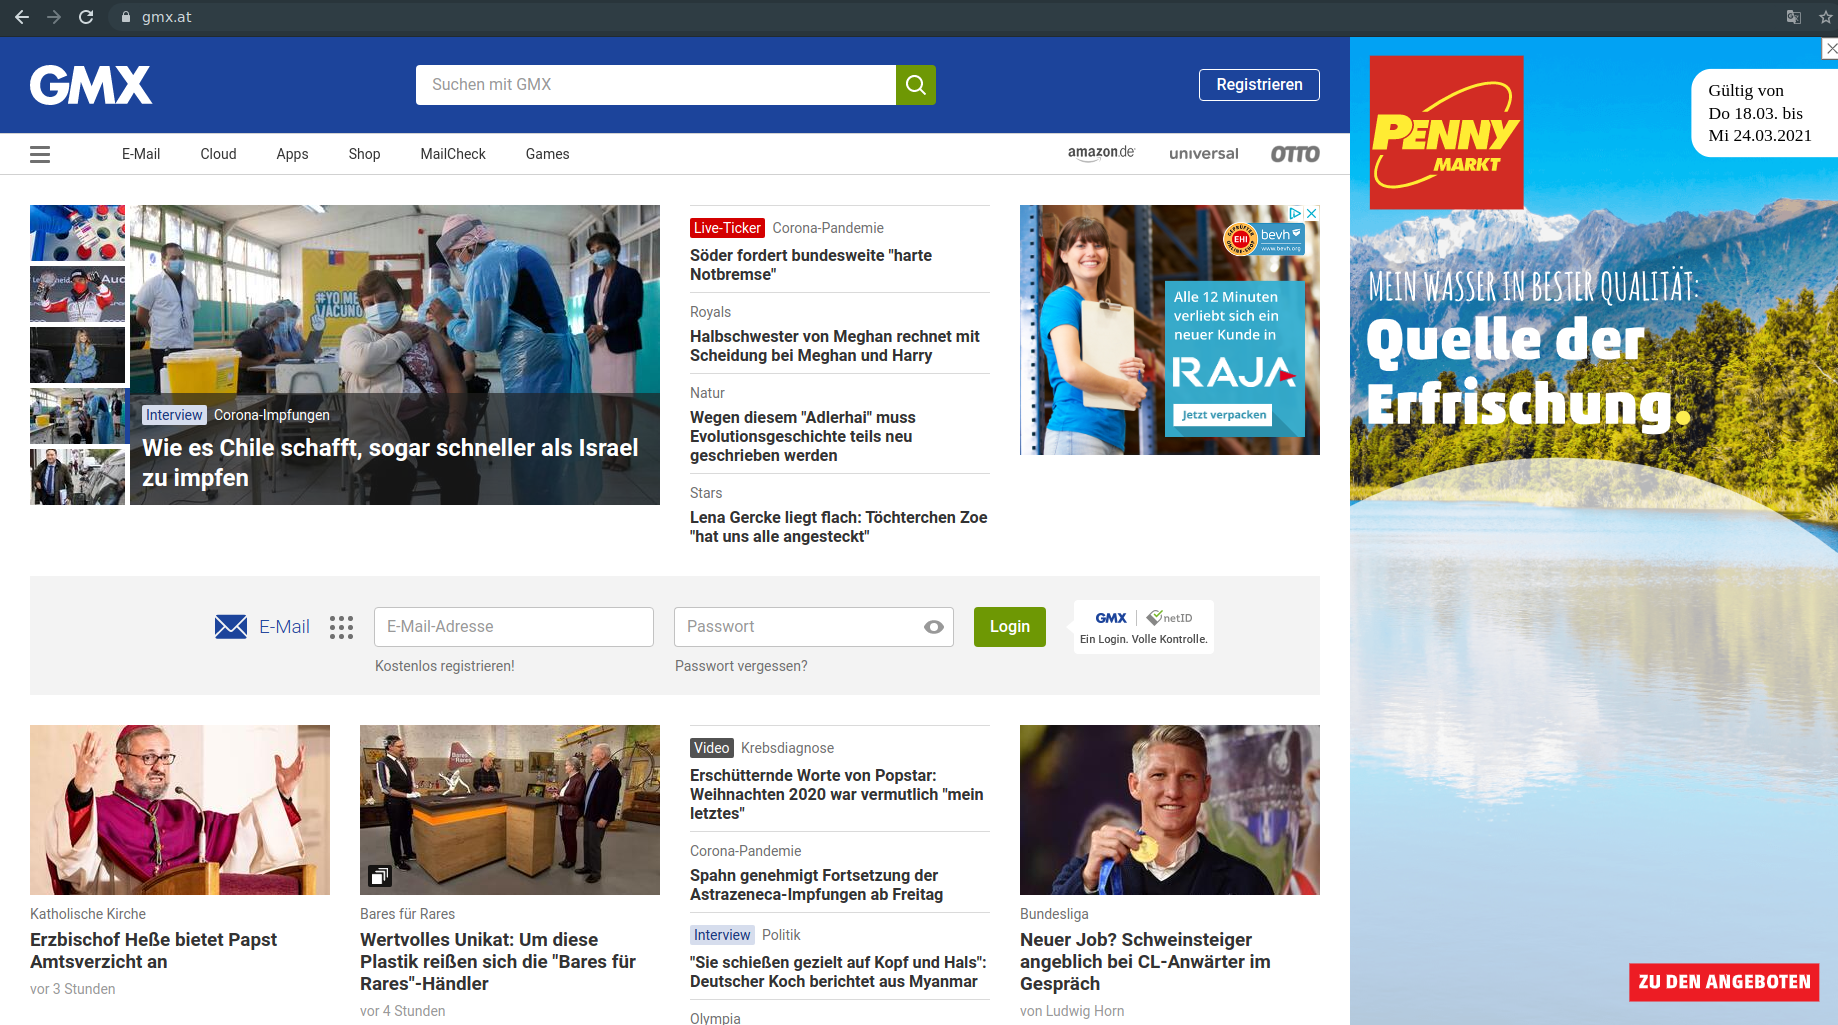
\includegraphics[width=400px]{./img/gmxat.png}
\end{center}

\subsubsection{Nielsen-Heuristiken}
\label{sec:org24dd2ee}

Obwohl sich die Seite an viele Design-Heuristiken wie gängige
Design-Standards (Logo in der linken oberen Ecke,
Registrier-Button rechts oben) hält, fällt mein Hauptkritikpunkt
unter den Punkt "\#8 Aesthetic and minimalist design" der
Nielsen-Heuristiken. Darunter leidet auch die Effizienz beim
Benützen des Webservices (\#7 Flexibility and efficiency of use).

\subsubsection{2 Verbesserungen}
\label{sec:org954f426}
\begin{enumerate}
\item Erste Verbesserung wäre eine Reduktion der Text- und
Bildflächen rund um den Login-Bereich inklusive größerer
Abstände zwischen den einzelnen Flächen und dem Login-Bereich,
um diesen besser hervorzuheben und leichter identifizierbar zu
machen.
\item Zweite Verbesserung wäre ein konsistentes Design in der
Anordung dieser verbliebenen Text- und Bildflächen, um die
gesamte Seite ansprechender zu machen. Dazu gehört auch eine
Bildauswahl zu den einzelnen Werbungen und Newsartikeln, die
nicht dem Zufall überlassen ist, sondern unter Berücksichtigung
der anderen Flächen gemacht wirds. Das betrifft vor allem die
Farben. Die Bilder sollten untereinander abgestimmt
sein. Bilder mit zu vielen Details, in die man erst
hineinzoomen muss, sollten dabei ohnehin vermieden werden.
\end{enumerate}
\end{document}
